\textbf{2.3-1}
Using Figure 2.4 as a model, illustrate the operation of merge sort on an array 
initially containing the sequence $<3, 41, 52, 26, 38, 57, 9, 49>$. \\
\begin{figure}[h]
    \centering
    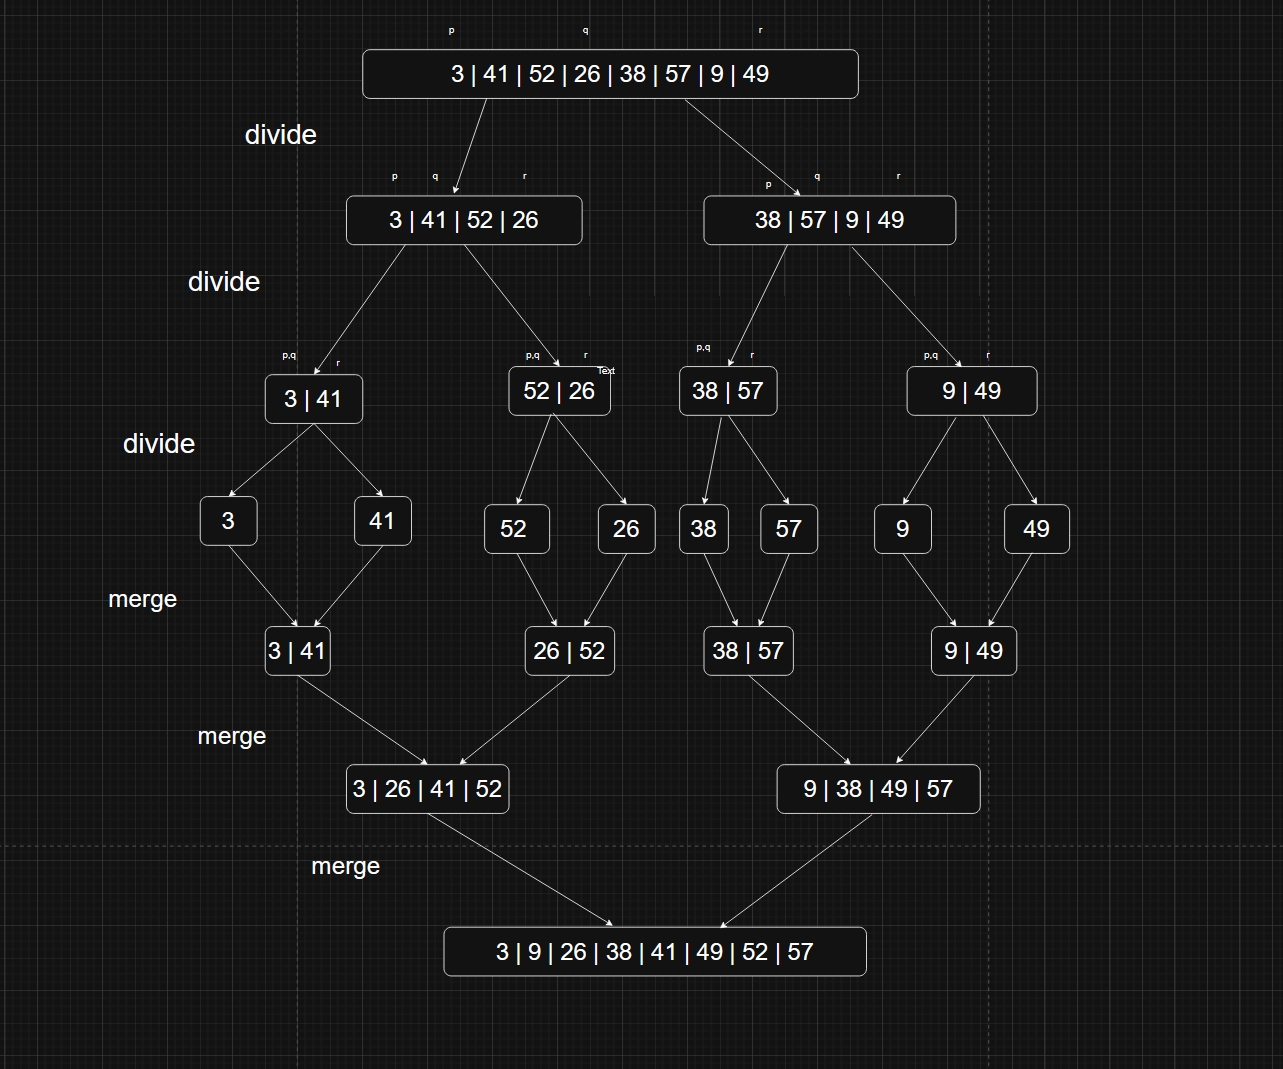
\includegraphics[width=0.6\textwidth]{./chapter2/2_3diagram.png}
\end{figure} \\

\textbf{2.3-2}

This test in line 1 of the MERGE-SORT procedure reads ``if $p \geq r$'' rather than
``if $p \neq r$.'' If MERGE-SORT is called with $p > r$, then the subarray
$A[p:r]$ is empty. Argue that as long as the initial call of
$\text{MERGE-SORT}(A,1,n)$ has $n \geq 1$, the test ``if $p \neq r$'' suffices
to ensure that no recursive call has $p > r$.

Given that the initial call of MERGE-SORT has $p = 1$ and $r = n$ where
$n \geq 1$, we must show that the test $p \neq r$ suffices to ensure that no
recursive call has $p > r$. From the initial call there are two cases:

\begin{enumerate}
\item $n = 1$

In this scenario, the function would not return since $1 \neq 1$ is false.
It would compute
\[
q = \frac{1 + 1}{2} = 1
\]

It then calls two more MERGE-SORT operations:

\[
\text{MERGE-SORT}(A,1,1)
\]

(which is the same as the initial call, causing infinite recursion), and

\[
\text{MERGE-SORT}(A,2,1)
\]

which has $p > r$. Therefore the claim that no recursive call has $p > r$
is false, and thus we have shown that $p \neq r$ does not suffice.

\item $n > 1$

There is no need to explore this case since case 1 already disproves the
argument.
\end{enumerate}

\textbf{2.3-3}

State a loop invariant for the while loop of lines 12-18 of the MERGE procedure. 
Show how to use it, along with the while loops of lines 20-23 and 24-27, to prove 
that the MERGE procedure is correct. 

\begin{description}
\item{Loop Invariant Statment: } 
At the start of each iteration of the loop (lines 12-18):
    The subarray A[p..k-1] contains the k-p smallest elements of L and R in sorted order.

\item{Initialization: } Before the first iteration:
. k=p
. The subarray A[p..k-1] is empty
An empty array is trivially sorted and contains the 0 smallest elements of L and R.
Therefore the invariant holds before the loop begins. 

\item{Maintenance: } Assume the invariant holds at the start of an iteration.
The algorithm compares:
. L[i]
. R[j]

This causes 2 cases:

Case 1
if L[i] $\leq$ R[j]
. A[k] = L[i]
. increment i
Since L[i] is the smallest remaining element, placing it next preserves the sorted order. 

Case 2
if R[j] < L[i]
. A[k] = R[j]
. increment j

Since the smallest ramining element is placed next. 

Then after either case:
. k is incremented
. A[p..k-1] still contains the smallest elements in sorted order
Thus the invariant is perserved.

\item{Termination: } The loop stops when either
. i = nL (left array exhausted) or
. j = nR (right array exhausted)
At this moment:
A[p..k-1] containse the smallest elements from L and R in sorted order, b one subarray may still conatin remaining elements.

\item{The Clean Up: } Two loops copy the remaining elements:

If left array remains
Lines 20-23 copy remaining L[i..nL-1] into A.
If right array remains
Lines 24-27 copy remaining R[j..nR-1] into A.
Because:
. L and R are already sorted
. All remaining elements are greater than the elements already placed
Thus appending them preserves the sorted order.

\end{description}


\textbf{2.3-4}

Use mathmatical induction to show that when $n \geq 2$ is an exact power of 2, the
solution of the recurrence \\
$T(n)=\begin{cases}
2 & :n=2, \\
2T(n/2)+n & :n > 2
\end{cases}$ \\
is T(n) = nlgn. \\

\begin{description}
\item{Base Case: } 
n = 2 so T(2)  = 2 and 2lg2 = 2(1) = 2 so this case holds. 

\item{Inductive Hypothesis: }
Assume that for the n = k case that 
$T(k)=\begin{cases}
2 & :k=2, \\
2T(k/2)+k & :k > 2
\end{cases}$ \\
is T(k) = klgk.

\item{Inductive Step: } Now we have to prove for the n = 2k case since  when $n \geq 2$ is an exact power of 2 is the restriction
so logically the next step from n = k that is an exact power of 2 is n = 2k 

$T(n)=\begin{cases}
2 & :n=2, \\
2T(n/2)+n & :n > 2
\end{cases}$ \\

we know that T(k) = klgk by inductive Hypothesis

if this is the base case we have already prove it so we now need to prove it in the case that 

n $>$ 2 or 2k $>$ 2  so we need to show 

2T($\frac{2k}{2}$) + 2k = (2k)lg(2k) $\rightarrow$ 2(T(k) + k) = 2(klg(2k))

and using the logarithmic product rule 
$\rightarrow$ 2(T(k) + k) = 2(k(lg(2) + lg(k)))

$\rightarrow$ 2(T(k) + k) = 2(k(1 + lg(k)))

communative property of addition
$\rightarrow$ 2(T(k) + k) = 2(k(lg(k) + 1))

distributive property of multiplication
$\rightarrow$ 2(T(k) + k) = 2(klg(k) + k)

using inductive hypothesis
$\rightarrow$ 2(T(k) + k) = 2(T(k) + k)

thus I have show using induction that 
when $n \geq 2$ is an exact power of 2, the
solution of the recurrence \\
$T(n)=\begin{cases}
2 & :n=2, \\
2T(n/2)+n & :n > 2
\end{cases}$ \\
is T(n) = nlgn. \\
\end{description}

\textbf{2.3-5}

You can also think of insertion sort as a recursive algorithm. In order to sort
A[1:n], recursively sort the subarray A[1:n-1] and then insert A[n] into the sorted subarray
A[1:n-1]. Write the code for this recurisve version of insertion sort. Give a recurrence for 
its worst-case run time. \\

\begin{verbatim}
def recursiveInsertionSort(array: list[int], n: int):
    if n <= 1:
        return

    # sort first n-1 elements
    recursiveInsertionSort(array, n-1)

    # insert last element into sorted part
    key = array[n-1]
    j = n-2

    while j >= 0 and array[j] > key:
        array[j+1] = array[j]
        j -= 1

    array[j+1] = key

\end{verbatim}

\textbf{2.3-6}

Referring back to the searching problem (see Exercise 2.1-4), observe that if the 
subarray being searched is already sorted, the searching algorithm can check the 
midpoint of the subarray against $v$ and eliminate half of the subarray from further
consideration. The binary search algorithm repeats this procedure, halving the 
size of the remaining portion of the subarray each time. Write pseudocode, either 
iterative or recursive, for binary search. Argue that the worst-case running time of 
binary search is  $\theta(lgn)$. \\

\begin{verbatim}
def search(target, a):
    n: int = len(a)
    l: int = 0
    r: int = n-1
    
    print(a)
    
    while (l <= r):
        m: int = (l+r) // 2
        print(m)
        val: int = a[m]
        
        if val == target:
            return m
        elif target > val:
            l = m+1
        else:
            r = m-1
            
    return -1
\end{verbatim}

The reason that the worst case is $\theta(lgn)$ is because of the way binary search works
so every time you check for the target you split the array you are searching in in half.
this creates a tree that splits as it goes doewn so say you have an array with 10 elements then
on the first iterations you check the middle at index 4. you then can either go left our right depending
on the target either way you end up with a new array of either 4 or 5 (half or a little less thann half)
you continue this untill you hit a array of 1 element. so it would shrink like $10 -> 5 -> 2 -> 1$ and 
$\theta(lgn(10)) = $ $3$--$4$  \\

\textbf{2.3-7}

The while loop of lines 5-7 of the INSERTION-SORT procedure in Section 2.1
uses a linear search to scan (backward) throught the sorted subarray A[1:j-1].
What if insertion sort used a binary search (Exercise 2.3-6) instead of a linear
search? Whould that imporove the overall worst-case run time to $\theta(nlgn)$? \\

No, because while binary search reduces the number of comparisons 
needed to find the correct position from $\theta(n)$ to $\theta(lg n)$, 
the shifting of elements in the inner loop is still $\theta(n)$ per iteration in 
the worst case. Since the shifting dominates, the overall worst case runtime 
remains $\theta(n^2)$\\

\textbf{2.3-8}

Write the algorithum that, given a set S of n integers and another integer x, determines whether S contains two elements
that sum to exactly x. Your algorithum should take $\theta(nlgn)$ time in the worst case. \\

\begin{verbatim}
from xmlrpc.client import boolean


def mergeSort(nums: list[int], l: int, r: int) -> list[int]:
  if not nums or l > r:
    return []
  if l == r:
    return [nums[l]]

  m: int = (l+r) // 2
  leftNums: list[int] = mergeSort(nums, l, m)
  rightNums: list[int] = mergeSort(nums, m+1, r)
  return merge(leftNums, rightNums)

def merge(nums1: list[int], nums2: list[int]) -> list[int]:
  # nums1
  i: int = 0
  n: int = len(nums1)

  # nums2
  j: int = 0
  m: int = len(nums2)

  res: list[int] = []

  while (i < n and j < m):
    if (nums1[i] <= nums2[j]):
      res.append(nums1[i])
      i += 1
    else:
      res.append(nums2[j])
      j += 1
  
  if i >= n:
    res.extend(nums2[j:m])
  else:
    res.extend(nums1[i:n])
  
  return res

# assumes a sorted array (if num at i then doesn't count cuz that is the other num's index)
def binarySearch(nums: list[int], i: int, x: int) -> bool:
  l: int = 0
  r: int = len(nums)-1

  while(l < r):
    m: int = (l+r)//2
    num: int = nums[m]

    if (num == x and i != m):
      return True
    elif (num == x and i == m):
      left = nums[i-1] if i > 0 else None
      right = nums[i+1] if i < r else None
      if left == num or right == num:
        return True
      else:
        return False
    elif (num > x):
      r = m
    else:
      l = m+1

  return False

# function that determines if nums contains 2 elements that sum to x
def containsTwoElementsSum(nums: list[int], x: int) -> boolean:
  n: int = len(nums)

  if n < 2:
    return False

  sortedNums: list[int] = mergeSort(nums, 0, len(nums)-1)
  for i in range(len(nums)):
    num: int = nums[i]
    if (binarySearch(nums, i, x-num)):
      return True
    
  return False

array: list[int] = [100, 43, 54, 23, 67, 1, 9, 413, 456, 21, 46, 80, 70]
sortedArray: list[int] = mergeSort(array, 0, len(array)-1)

print(array)
print(sortedArray)
print(containsTwoElementsSum(sortedArray, 18))
\end{verbatim}



